\chapter{Results and Discussion}\label{chapter:results}

When testing the naive metric against the test data, obtained from the hand posture evaluation of the pilot study, it can be seen that the computed metric values do correlate with the user rating. Figure \ref{fig:testDataNaive} shows an \texttt{R} plot of the data. The dots represent the individual hand posture ratings and the line shows the smoothed conditional mean, calculated by the \texttt{geom\_smooth} function. The computed Pearson correlation of -0.6651999 confirms this and the p-value of 6.73e-9 shows that the correlation is highly significant (taking 0.01 as a threshold for p-value significance). 

\begin{figure}[h]
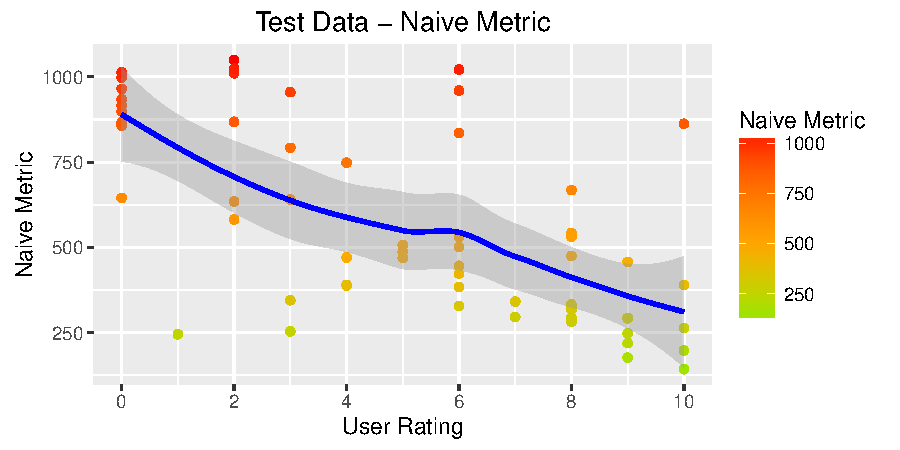
\includegraphics[width=\textwidth]{TestDataNaive}
\caption{Naive Metric and User Rating in Test Data.}
\label{fig:testDataNaive}
\end{figure}

For improving the metric, finding the best fitting 17 weighting coefficients can be reduced to a curve fitting problem with 17 unknowns. Therefore we used the least squares algorithm on the first 250 data sets from the second user study to fit the comfort/discomfort metric values to the user ratings. This was done with the \texttt{lsfit} function in \texttt{R}. Afterwards we tested our results against the remaining 60 data sets from the pilot study to validate them. For this, we decided to combine comfort and discomfort, as we suspected both comfort and discomfort to affect performance.

\begin{table}
\centering
\caption{Weighting Coefficients of different Metric Components}
\label{tab:coeff}
\begin{tabular}{|c|l|l|l|l|l|} \hline
 &Thumb&Index&Middle&Ring&Pinky\\ \hline
RRP&0.631&-1.837&1.176&-3.021&1.288\\ \hline
IFA&-&0.547&0.216&1.670&-0.864\\ \hline
HE&-&-1.637&-2.685&10.401&-1.837\\ \hline
FA&-&-0.864&-3.857&0.0388&2.517\\
\hline\end{tabular}
\end{table}

The computed coefficients can be taken from Table \ref{tab:coeff}. When looking at the values, following points can be observed: 
\begin{enumerate}
	\item The values are very noisy, this is probably due to the small number of participants and data samples. 
	\item The inter finger angle component seems to be the most important one, as the IFA coefficients are the least noisy.
	\item For most hand postures abduction and hyperextension are widely ignored by users, therefore their coefficients are highly noisy. 
\end{enumerate}

\begin{figure}[h]
\centering
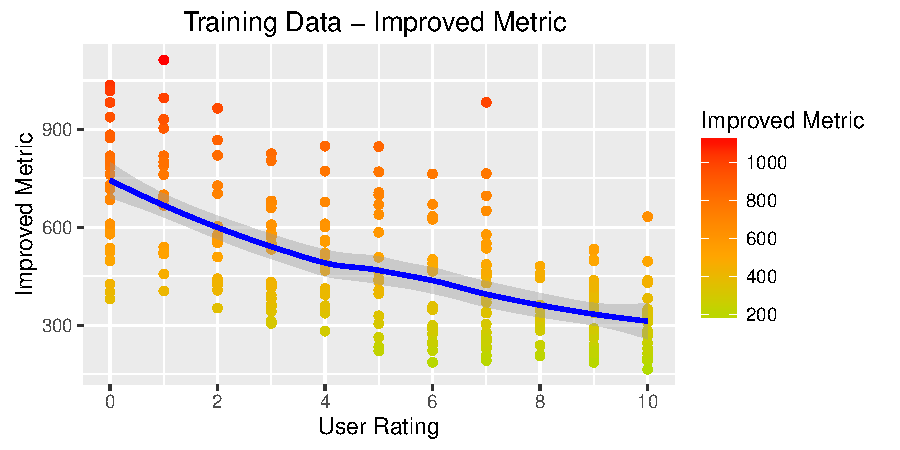
\includegraphics[width=\textwidth]{TrainingDataImproved}
\caption{Improved Metric and User Rating in Training Data.}
\label{fig:trainingData}
\end{figure}

Unsurprisingly, there was a correlation in the training data between the user rating and our improved metric, generated using this very data (Figure \ref{fig:trainingData}). Despite its high significance due to a p-value of < 2.2e-16, the correlation found was still not perfect, having a value of -0.6453242. For this we suspect multiple reasons: 

\begin{itemize}
	\item The participants most likely had differences in anatomy and mindset, which caused them to subjectively rate comparable postures differently. 
	\item There was little time for subjects to give their rating. Therefore long time discomfort symptoms, like pain or cramping, might not have been experienced. 
	\item The subjects could only rate the hands of continuous comfort/discomfort on a scale with 11 discrete steps, which potentially introduced some additional error.
\end{itemize}

\begin{figure}[h]
\centering
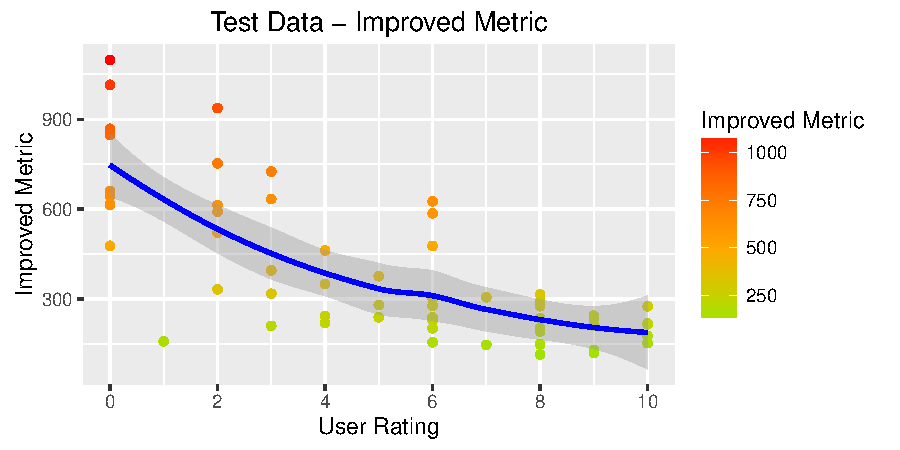
\includegraphics[width=\textwidth]{TestDataImproved}
\caption{Improved Metric and User Rating in Test Data.}
\label{fig:testData}
\end{figure}

Even though the improved metric was created using a limited set of training data, it yielded an even better significant correlation of -0.748993 when applied to the test data (Figure \ref{fig:testData}, p-value: 5.89e-12). This indicates that the improved metric is a good extrapolation of the training data. Compared to the naive metric (Figure \ref{fig:testDataNaive}), there is only minor difference on first sight. However, the improved metric reduced the variance in the data, resulting in a better correlation and p-value.

\begin{figure}[h]
\centering
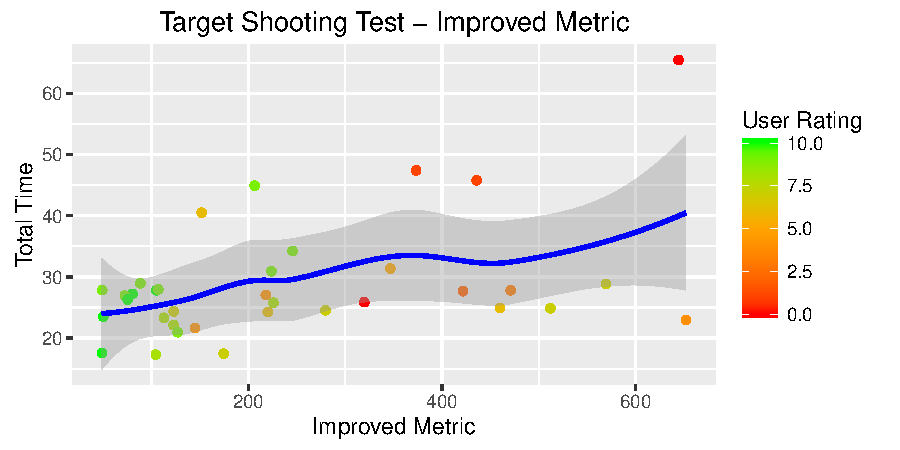
\includegraphics[width=\textwidth]{TargetShooting}
\caption{Improved Metric Value and Total Task Time in Target Shooting.}
\label{fig:targetShooting}
\end{figure}

The results from the target shooting task (Figure \ref{fig:targetShooting}) show a significant correlation of -0.66519 (p-value: 6.73e-9) that indicates that comfort and discomfort, as measured by our metric, do affect the performance and precision in context of hand postures. This strengthens the conclusion of Short et al. \cite{short1999precision}, that more comfortable postures generally create greater accuracy. However, the credibility of our results is limited by the relatively small number of participants. Thus further work is required before strong conclusions can be made.